\documentclass[../main.tex]{subfiles}
\graphicspath{{\subfix{../images/}}}


\begin{document}
% AIS
%%%%%%%%%%%%%%%%%%%%%%%%%%%%%%%%%%%%%%%%%%%%%%%%%%%%%%%%%%%%%%%%%%%%%%%%%%%%%%%
The Baltic Sea with an approximate surface area of 420,000 km$^2$ is rather small compared to other seas and navigating in the Baltic Sea is often confined to fairways, especially when getting closer to land and travelling in the archipelago. This creates highways of vessel traffic coming from and going to the many ports in the Baltic Sea merging into one another at some point during the voyage. This is even more evident in the winter months when there are restrictions on where vessels are allowed to navigate due to the ice, which is governed by the Finnish and Swedish authorities. During the winter months, vessels might also be required to get help from an icebreaker to enter the port, and with only around 30 operational icebreakers in the Baltic Sea could even create queues to get assistance where vessels have to anchor until assistance arrives. Other characteristics are the areas of international waters in the Baltic Sea; vessels travelling from and to the east part of the Baltic Sea often use these areas as an example. To enter the Baltic Sea from the Atlantic, all vessels have to travel through the Danish straits and Kattegat.

The past years, approximately 90 \% of all import and export of Finland was done by sea \cite{SVRY_2022}. There is no question about the importance of sea transports and maintaining efficient operations at sea and at port is of interest for all parties, especially in Finland where most of all imports and exports passes through ports at some point during the transportation.

One important port for the Finnish industry and economy is the Port of Naantali. Located close the city of Turku and having a central location in the Baltic Sea it was deemed to be a suitable candidate for the thesis.

\subsection{Automatic identification system}

Automatic identification system (\textit{AIS}) was introduced by the International Maritime Organization (\textit{IMO}) in the early 2000's in accordance with the Safety of Life at Sea (\textit{SOLAS}) treaty as an open communication tool for all maritime traffic. The main objectives of the treaty is to improve the safety of life at sea, protection of the marine environment and safety and efficiency of navigation \cite{IMO_2015}. In its general operating form, AIS operates on two VHF channels and all vessels or base stations within the vessels transmission range receive the messages transmitted and vice versa the vessel receives all messages broadcasted in its receiving range. The broadcasting is based on Self-organized Time Division Multiple Access (\textit{(S)TDMA}) with a minimum of 2000 time slots per minute broadcasting capacity rate and the ship-to-ship communication for vessels closer to each other, takes precedence over vessels farther away from one another, which allows for sharing time slots, and thus overloading the available time slots \cite{IMO_2015}.

The IMO requires in accordance with regulation V/19 of SOLAS, that all vessels with a gross tonnage of 300 or more on international voyages, cargo vessels of 500 gross tonnage or more not on international voyages and all passenger vessel disregarding the gross tonnage to be equipped with an AIS. Further, the EU requires new-built fishing vessels longer than 15 meters to be fitted with an AIS from November 2010 and existing vessels to install a AIS by May 2014 at the latest \cite{EU_2011}. There are two types of AIS, Class A and Class B. Class A transceiver are the more common and are compliant with the IMO regulations whereas Class B transceivers are not subject to the full IMO AIS requirements. Class B transceivers are typically simpler, of lower cost and installed on smaller vessels of one's own choosing for improving the situational awareness. Class A transceivers take precedence over Class B transceivers when broadcasting.

The vessels onboard sensors and positioning systems interface with the AIS to allow for communicating the status of the vessel, both static and dynamic information. AIS also allows for voyage related information and safety-related information to be transmitted via the system, see Table \ref{tab:ais-data}. The AIS guidelines requires that there is a minimum display and keyboard for input and receiving data, for updating information manually and retrieving data received via AIS. Some data for the AIS is entered only once, other has to be entered for every voyage and other data will be automatically gathered from the vessels onboard sensors.

The information received by the AIS does not provide the full situational picture of the vessels surroundings and should only be used as a navigational and situational awareness aid.

\begin{figure}[H]
\centering
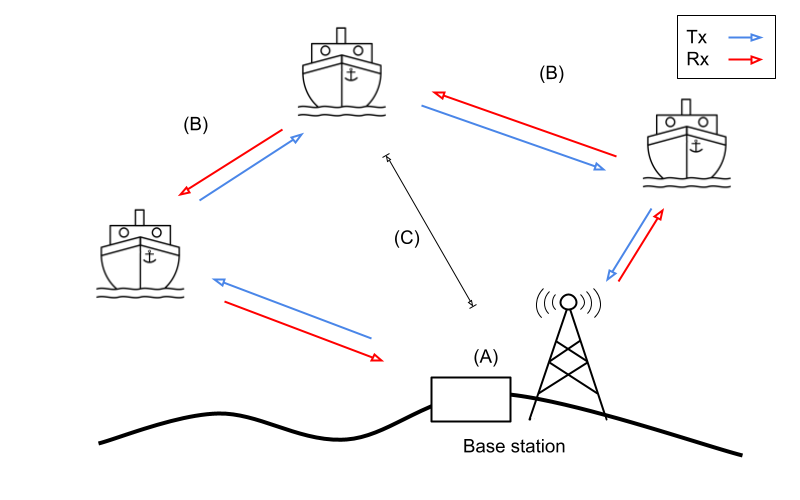
\includegraphics[scale=.5]{AIS-SOP.png}
\caption{(A) Base station transmits information about other vessels, port data and possible hazards. Base station receives information from all vessels in range. (B) Ship-to-ship communication. Vessel broadcasts its current state (identifier, speed over ground, course over ground etc.) and receives data from all vessels in range, only limited by the number of possible time slots available. (C) Vessel outside the range of broadcasting AIS data to the base station, still broadcasts information to other vessels.}
\label{fig:ais-sop}
\end{figure}

The AIS integrated checks for data integrity, built-in integrity test (\textit{BIIT}), is not capable of validating data, for example a non-functional sensor will report as not available to the AIS. This can introduce faulty data being broadcasted to surrounding vessels and could create dangerous situations.

The nature of AIS being unencrypted and unauthenticated with the fact that there is no data validation before transmitting does entail that the veracity of the data is poor. The information available through AIS should not be trusted by itself and it is up too the OOW to safely operate the vessel and ensure safe navigation for the vessel and vessels in its surroundings. 

The information available to transmit over AIS is divided into three groups; static, dynamic and voyage-related.

\begin{table}[H]
\centering
\begin{tabular}{|m{5cm}|m{9cm}|}
\hline
\rowcolor[HTML]{C0C0C0} 
\multicolumn{1}{|c|}{\cellcolor[HTML]{C0C0C0}\textbf{Data}}  & \multicolumn{1}{c|}{\cellcolor[HTML]{C0C0C0}\textbf{Description}}                 \\ \hline
\rowcolor[HTML]{C0C0C0} 
\textbf{Static}                                              &                                                                                   \\ \hline
Maritime Mobile Service Identity (MMSI)                      & Set on installation, can change during vessels operational lifespan               \\ \hline
%\rowcolor[HTML]{EFEFEF} 
Call sign and name                                           & Set on installation, can change during vessels operational lifespan               \\ \hline
IMO number                                                   & Set on installation                                                               \\ \hline
%\rowcolor[HTML]{EFEFEF} 
Length and beam                                              & Set on installation or if changed                                                 \\ \hline
Type of ship                                                 & Selected from list of predefined values                                           \\ \hline
%\rowcolor[HTML]{EFEFEF} 
Location of electronic positioning system                    & Set on installation, can be changed                                               \\ \hline
\rowcolor[HTML]{C0C0C0} 
\textbf{Dynamic}                                             &                                                                                   \\ \hline
Ships position with accuracy indication and integrity status & Automatically updated from the position sensor                                    \\ \hline
%\rowcolor[HTML]{EFEFEF} 
Position time stamp in UTC                                   & Automatically updated from the main position sensor                               \\ \hline
Course over ground (COG)                                     & Automatically updated from the main position sensor if available                  \\ \hline
%\rowcolor[HTML]{EFEFEF} 
Speed over ground (SOG)                                      & Automatically updated from the main position sensor                               \\ \hline
Heading                                                      & Automatically updated from the vessels heading sensor                             \\ \hline
%\rowcolor[HTML]{EFEFEF} 
Navigational status                                          & Manually entered by the OOW as needed                                             \\ \hline
Rate of turn (ROT)                                           & Automatically updated from the vessels ROT sensor or from the vessels gyro        \\ \hline
\rowcolor[HTML]{C0C0C0} 
\textbf{Voyage-related}                                      &                                                                                   \\ \hline
Draught                                                      & Manually entered at the start of the voyage                                       \\ \hline
%\rowcolor[HTML]{EFEFEF} 
Hazardous cargo (type)                                       & Manually entered at the start of the voyage confirming the presence of such cargo \\ \hline
Destination and ETA                                          & Manually entered at the start of the voyage and updates as needed                 \\ \hline
%\rowcolor[HTML]{EFEFEF} 
Route plan (waypoints)                                       & Manually entered at the start of the voyage                                       \\ \hline
\rowcolor[HTML]{C0C0C0} 
\textbf{Safety-related}                                      &                                                                                   \\ \hline
Short safety-related messages                                & Free format manually entered broadcasted to specific receiver or all vessels      \\ \hline
\end{tabular}
\caption{AIS data content and description, source \cite{IMO_2015}.}
\label{tab:ais-data}
\end{table}

Depending on the type of message sent by the AIS, the rate at which the AIS transmits messages autonomously changes. For static and voyage-related data the interval is six minutes between messages or at the request of another user. Dynamic information on the other hand takes the vessels current navigational status into consideration at which rate to transmit messages.

The different states of a vessel and at which rate it will transmit autonomously AIS messages with dynamic information can be seen in Table \ref{tab:ais-rates}. Faster moving vessels will broadcast its location and trajectory more frequently as a faster moving vessel will cover longer distances and can alter its course more over a shorter time. It is still important for the OOW to understand that not all vessels will be transmitting AIS data and therefore AIS is not guaranteed to provide a complete overview of the surroundings. It is also not guaranteed that other vessels are receiving AIS data and could therefore be a risk factor. 

\begin{table}[H]
\centering
\begin{tabular}{|m{7cm}|m{4cm}|}
\hline
\rowcolor[HTML]{C0C0C0} 
\textbf{Vessel state}                                  & \textbf{General reporting interval} \\ \hline
At anchor or moored and not moving faster than 3 knots & 3 min                               \\ \hline
At anchor or moored and moving faster than 3 knots     & 10 s                                \\ \hline
0-14 knots                                             & 10 s                                \\ \hline
Changing course at 0-14 knots                          & 3 1/3 s                             \\ \hline
14-23 knots                                            & 6 s                                 \\ \hline
Changing course at 14-23 knots                         & 2 s                                 \\ \hline
Faster than 23 knots                                   & 2 s                                 \\ \hline
Changing course at more than 23 knots                  & 2 s                                 \\ \hline
\end{tabular}
\caption{AIS message broadcast interval for dynamic information for class A vessels \cite{IMO_2015}.}
\label{tab:ais-rates}
\end{table}


\subsubsection{Estimated Time of Arrival}

Estimated time of arrival is the estimated time when a vessel will reach its destination, typically transmitted to the correct authorities 24 to 72 hours before arrival \cite{Veenstra_2021, EU_2009}. The means of communicating this ETA varies and the accuracy of the ETA is not guaranteed to be within any margin of error. Ports, being very complex infrastructures with many moving parts, has to operate with certain uncertainties of vessels arrival times and required demands and it is essential to plan port operations for a 24-hour period at a minimum to ensure smooth operations \cite{Fancello_2011}. All uncertainties that can delay or alter any operations at one port are therefore a risk that can delay and disrupt all operations for not only the port in question but also all other ports that have any relations to the port.

There are many different practices for relaying the ETA to the correct authorities, for example via the AIS, phones and email. However, a study by \Citeauthor{Mokhtari_2008} \cite{Mokhtari_2008} discovered that almost a majority of the transmitted AIS messages had faulty or inaccurate data for the destination and ETA. Another risk discovered with the destination and ETA, when the data was available, was that it was not updated and thus could lead to more problems if any party thought the information to be true. An incorrect or inaccurate ETA could mean port authorities failing to plan its operations to handle incoming and outgoing traffic within the expected time.

\subsection{The Baltic Marine Environment Protection Commission}

The Baltic Marine Environment Protection Commission or Helsinki Commission (\textit{HELCOM}) as it is also known, was formed in 1974 parallel with the \textit{Convention on the Protection of the Marine Environment of the Baltic Sea}. The participating parties are Denmark, Estonia, the European Union, Finland, Germany, Latvia, Lithuania, Poland, Russia and Sweden with the goal to protect the marine environment from increasing exploitation and ensuring protection of the ecosystem in the Baltic Sea \cite{HELCOM_2014}.

\begin{figure}[H]
	\centering
	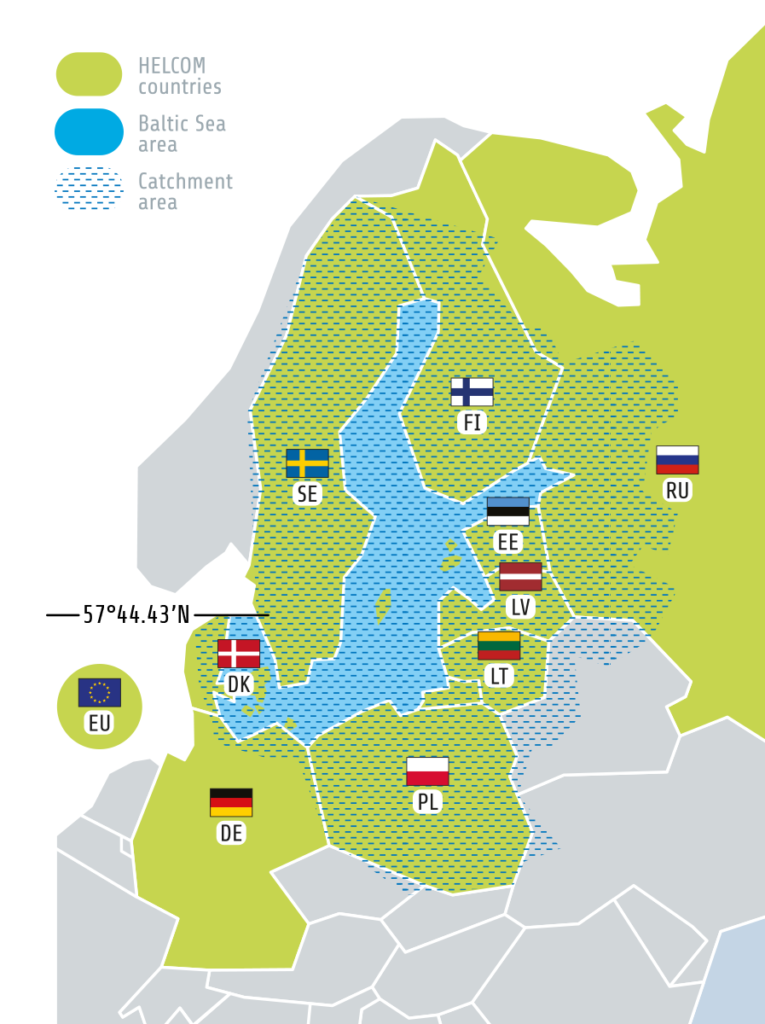
\includegraphics[scale=.3]{HELCOM_oper_area.png}
	\caption{Area of the Baltic Sea of the Helsinki Convention, source \protect\url{https://helcom.fi/about-us/}}
	\label{fig:helcom-area}
\end{figure}

\subsubsection{HELCOM dataset}

The HELCOM dataset consisting of AIS data, covers the period from January 2009 to December 2019. Each month for each year is stored as its own comma separated value \textit{.csv} file.

The AIS data in the HELCOM dataset has already been processed from what is originally transmitted from the AIS. All rows in the dataset has been made uniform to include the same data, every entry in the dataset contains exactly the same features. This has been possible by merging many different databases into one and this has also made it possible to cover the whole operating area of HELCOM, which includes all of the Baltic Sea seen in Figure \ref{fig:helcom-area}.

%
% Include small timewindow of helcom dataset mapped
%


\subsubsection{Description of HELCOM dataset features}

The HELCOM dataset have twelve unique features for each entry described in Table \ref{tabl:HELCOM-features}. The features are static, dynamic and voyage-related AIS data merged from multiple sources.

The combination of these features gives information about the vessels identification, position, time stamp, trajectory, draught and physical size. 

\begin{table}[H]
\centering
\begin{tabular}{|l|m{7cm}|l|}
\hline
\rowcolor[HTML]{C0C0C0}
\textbf{Name} & \textbf{Description}                                                  & \textbf{Value}             \\ \hline
timestamp     & Unix epoch time in milliseconds when AIS message was created          & Min 1230768000000          \\ \hline
mmsi          & Maritime Mobile Service Identities, unique for each vessel can change & 9 digit identifier         \\ \hline
lat           & Latitude position when AIS message was generated                      & Coordinate in WGS 84       \\ \hline
long          & Longitude position when AIS message was generated                     & Coordinate in WGS 84       \\ \hline
sog           & Speed over ground in knots                                            & 0.1 knot resolution        \\ \hline
cog           & Course over ground in degrees relative to true north                  & 0.1 degrees                \\ \hline
draught       & Vertical distance from waterline to the keel                          & 0.1 meters                 \\ \hline
dimBow        & Reference point for position of positioning system on the vessel      & Meters from bow            \\ \hline
dimPort       & Reference point for position of positioning system on the vessel      & Meters from port side      \\ \hline
dimStarboard  & Reference point for position of positioning system on the vessel      & Meters from starboard side \\ \hline
dimStern      & Reference point for position of positioning system on the vessel      & Meters from stern          \\ \hline
imo           & Unique identifier for each vessel, does not change                    & 7 digit identifier         \\ \hline
\end{tabular}
\caption{Variables in HELCOM data set and description.}
\label{tabl:HELCOM-features}
\end{table}

\subsubsection{Statistical information}
\label{sec:AIS-stat}
The HELCOM dataset covers a large window of time and gives an insight into historical vessel movements on the Baltic Sea. The dataset has been created by merging many databases and processing the data to create a uniform dataset for the whole period. In this dataset it is possible to find vessels movements on the Baltic Sea, where they are going and where they have been, by grouping the data by unique vessels and then order the data for each vessel in chronological order. It is not given that a vessel will have a contiguous timeline without gaps, this due to the possibility when a vessel has travelled outside the area covered by the AIS or have turned off their AIS for any reason. These gaps can be many months even years long and does not impact the quality of the routes. Smaller gaps in the timeline of a vessel does however impact the quality of the routes. There are many reasons for why vessels timelines can have smaller gaps, less than a couple of hours, and all of them will negatively impact the possibility of finding good routes. Some of the most likely reasons are malfunctioning AIS, the AIS has been turned off or the data received has been faulty and not stored.

\begin{figure}[H]
	\centering
	\includegraphics[scale=.45]{raw_example_many_vessel_routes_comingandgoing.png}
	\caption{Small window of time of raw AIS data from the HELCOM dataset. Coloured by unique vessels.}
	\label{fig:raw-ais-data}
\end{figure}

Figure \ref{fig:raw-ais-data} shows a small window of time from the HELCOM dataset of all AIS data. Only a fraction of this data is viable for further processing, but a first pass over the whole dataset is required to capture all possible vessels for each month.

The average speed over ground for routes going to the Port of Naantali seen in Figure \ref{fig:sog-dist}, indicates a even distribution of vessels travelling about 14 knots. This is expected from the types of vessels that are equipped with AIS and have been recorded in the dataset.

\begin{figure}[H]
	\centering
	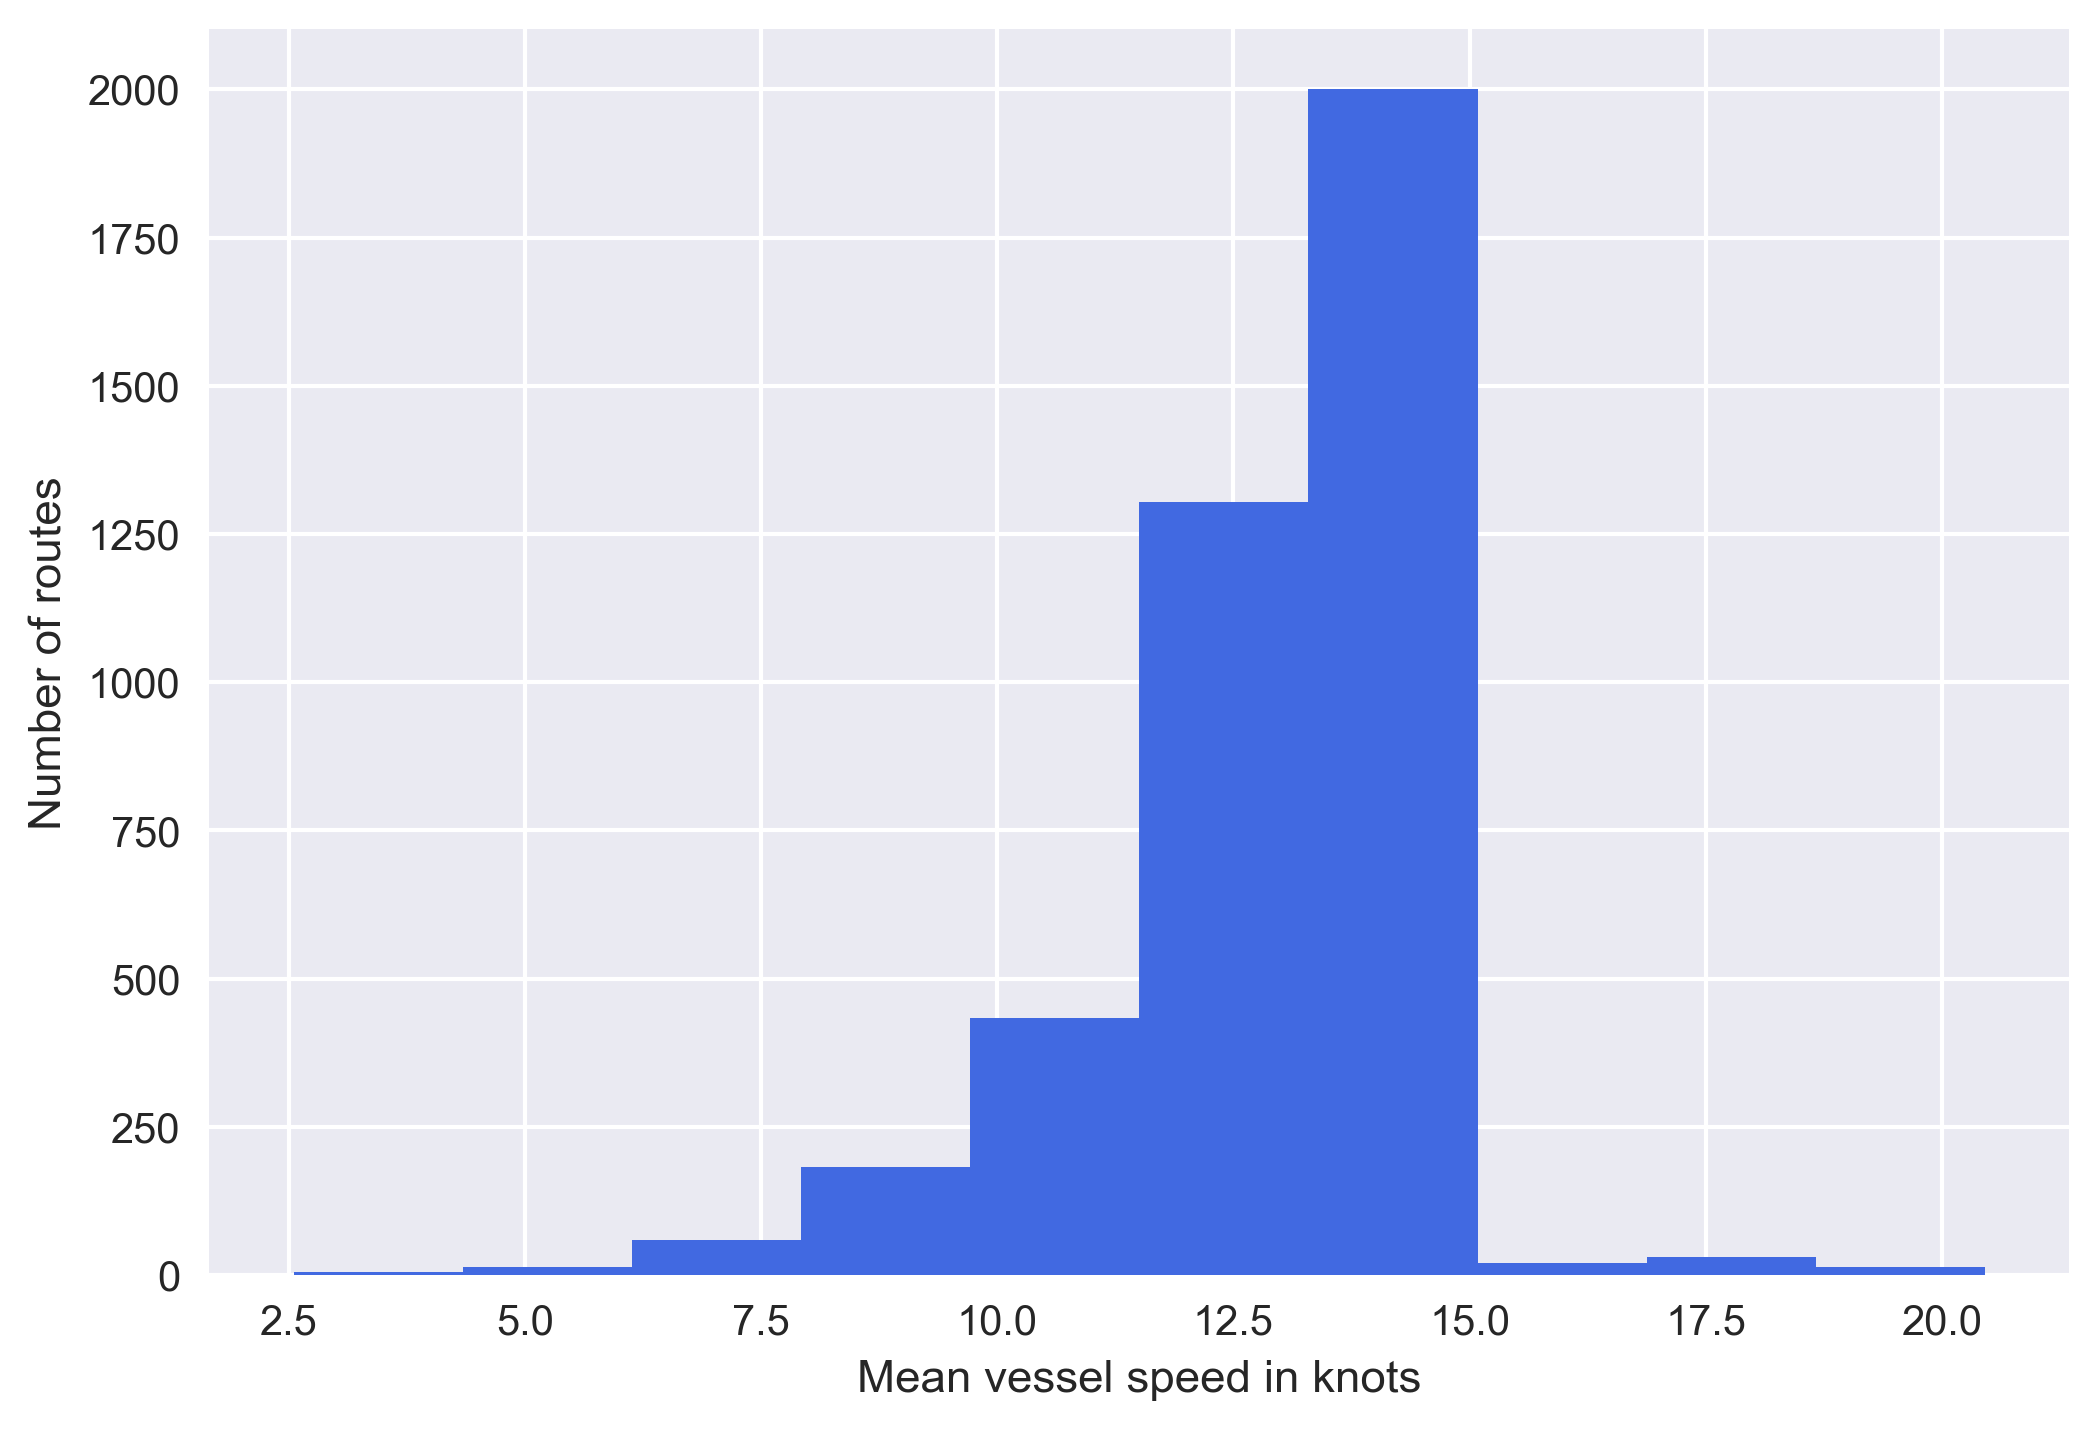
\includegraphics[scale=.6]{2009-2018-sog.png}
	\caption{Average vessel speed for a route for all routes used, from the period of 2009 to 2018.}
	\label{fig:sog-dist}
\end{figure}

The time difference between AIS messages does not correlate to what raw AIS transmission rates should be, see Table \ref{tab:ais-rates}. A concentration of time difference between one and four minutes is another indication of pre-processing done by HELCOM, as the timesteps compared are from windows of time where vessels have been under way during a route.

\begin{figure}[H]
	\centering
	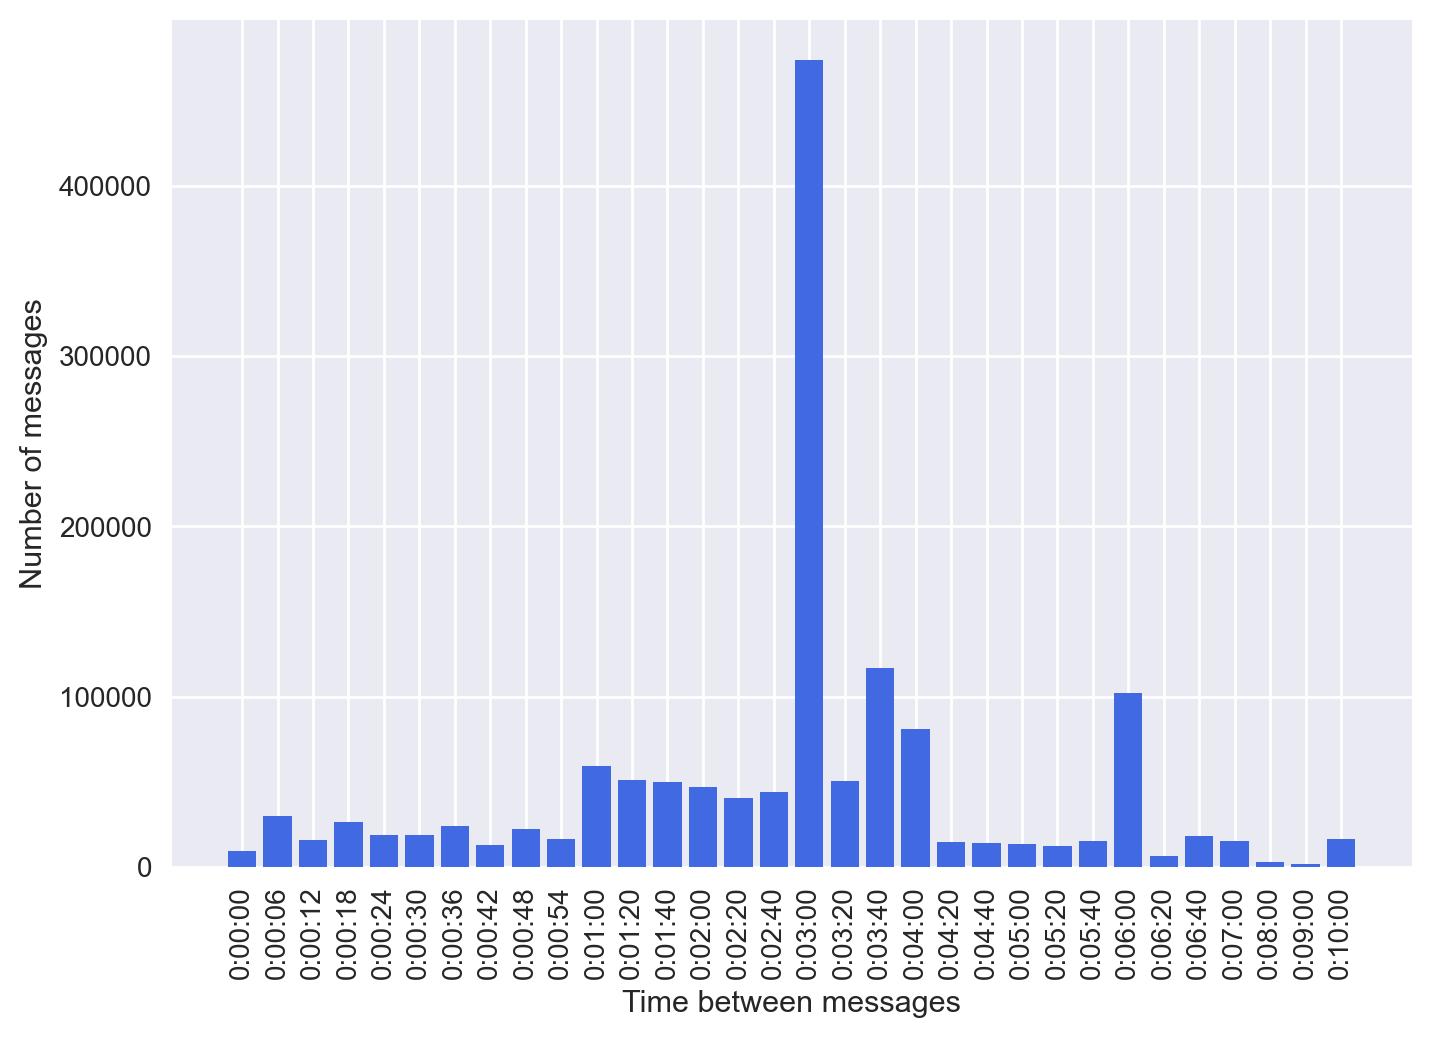
\includegraphics[scale=.6]{5y_ais_message_dist.png}
	\caption{Time difference between AIS messages for any routes found during a five year period. All time differences greater than ten minutes have been collected in the same bar.}
	\label{fig:ais-msg-dist}
\end{figure}


Vessels physical features and the grouping of different vessels by size. In Figure \ref{fig:vessel-classes} an example of one year of unique vessels which have visited the port of Naantali can be seen. Classifying vessels according to the physical size of the vessel has shown to be a efficient way of discerning different vessels capabilities of manoeuvring \cite{Jahn_2018}. It is expected that vessels of similar dimensions manoeuvre in a similar fashion. The classification was done by estimating different groups of vessels from their length and width, after which they were classified into classes according to the boxes seen in Figure \ref{fig:vessel-classes}.

\begin{figure}[H]
	\centering
	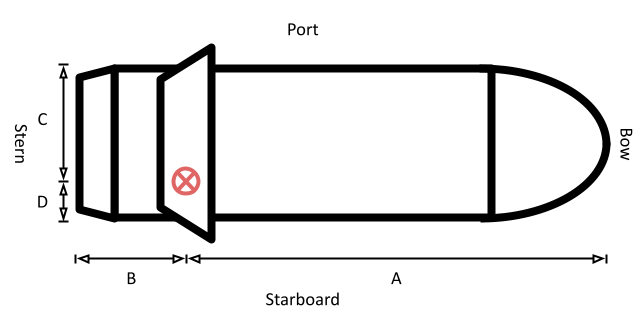
\includegraphics[scale=.5]{vessel-class-definition.png}
	\caption{Vessel class definition from HELCOM data, the positioning system marked with red. A is \textit{dimStern}, B is \textit{dimBow}, C is \textit{dimPort} and D is \textit{dimStarboard}.}
	\label{fig:vessel-class-def}
\end{figure}

\begin{figure}[H]
	\centering
	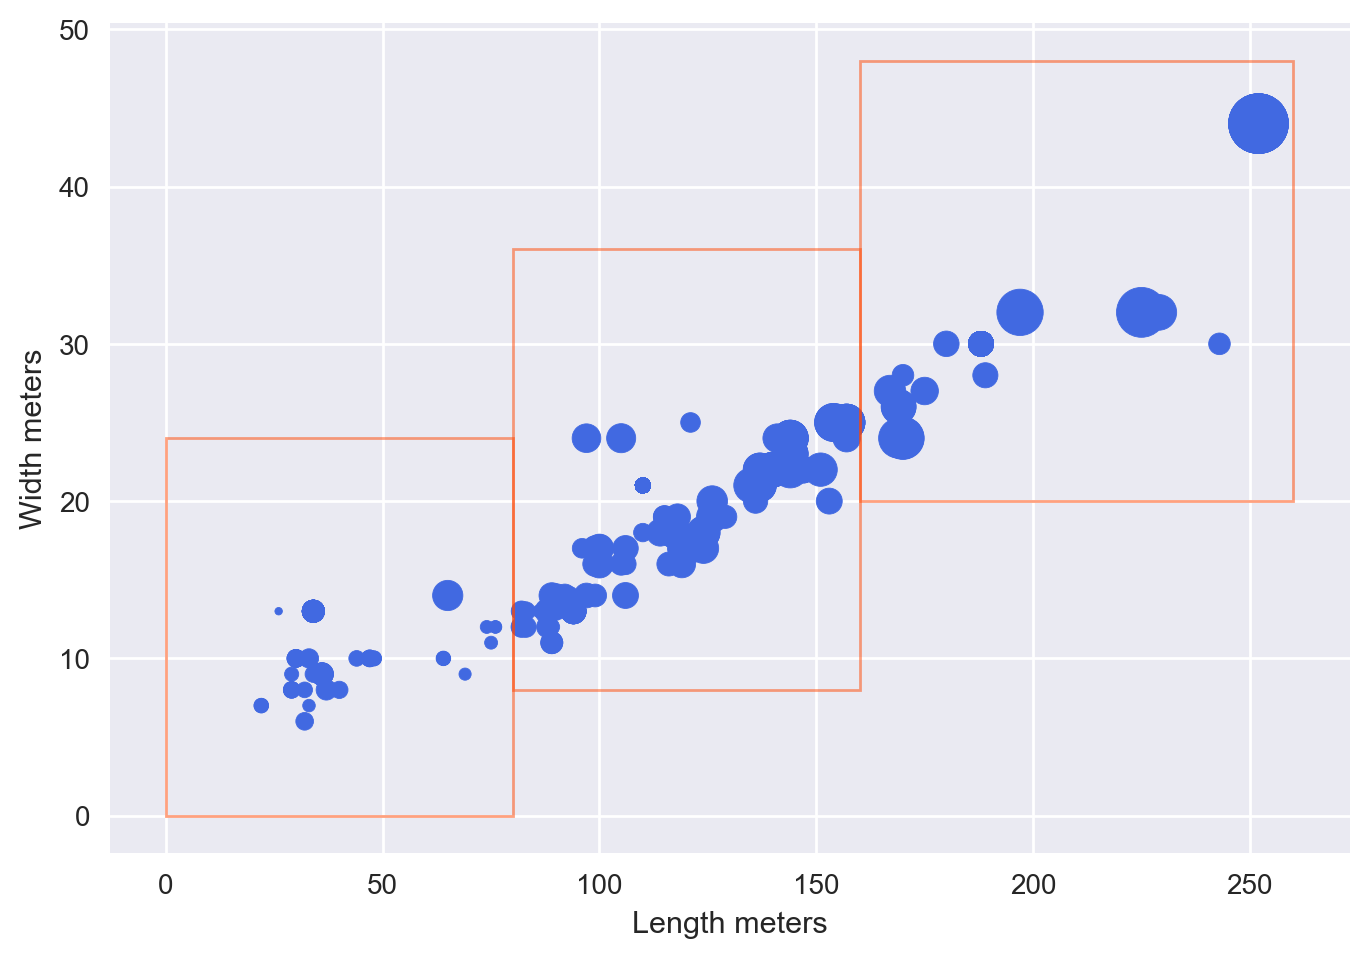
\includegraphics[scale=.5]{2015_ship_class.png}
	\caption{Defined vessel classes and distribution of all unique vessels for the year 2015. Size of the circle is related to the draught of the vessel.}
	\label{fig:vessel-classes}
\end{figure}


\subsection{Port of Naantali}

The Port of Naantali is a rather important and busy port in the Baltic Sea and it is considered one of Finlands most busy ports \cite{SVRY_2022}. With a reported total of over 8 million tonnes of cargo passing through the port and over 1,000 port calls during 2020 its logistical importance is of significance \cite{PoN_2021}. The port did at average for the years 2018 through 2020 handle at average 5,8 \% of all of Finlands transports by sea and combined with the port at Kilpilahti handled all of Finlands crude oil transport \cite{TRAFICOM_2021}.

This is also recognised in the HELCOM data by the amount of the data that has any connections to the Port of Naantali.

\begin{table}[H]
\centering
\begin{tabular}{|l|c|c|c|c|c|c|c|c|c|c|}
\hline
\rowcolor[HTML]{C0C0C0} 
\multicolumn{1}{|r|}{\cellcolor[HTML]{C0C0C0}\textbf{Year}} & \textbf{2009} & \textbf{2010} & \textbf{2011} & \textbf{2012} & \textbf{2013} & \textbf{2014} & \textbf{2015} & \textbf{2016} & \textbf{2017} & \textbf{2018} \\ \hline
\textbf{\% of data}                           & 8.21          & 7.16          & 7.30          & 13.19         & 12.30         & 12.30         & 12.30         & 10.17         & 10.87         & 10.61         \\ \hline
\end{tabular}
\caption{Total amount of vessel data with connection to the Port of Naantali for each year of the HELCOM data.}
\label{tab:HELCOM-data-percent}
\end{table}

The percentage of the data in Table \ref{tab:HELCOM-data-percent} is the complete timeline for each vessel that has at any point during the years visited the Port of Naantali, including other voyages that are not going and coming from the Port of Naantali. Only a fraction of this data is actual viable data for the routes, described in \ref{sec:algo-section}. Still, the fact that 10 \% on average of all data has any connection to the Port of Naantali further indicates its importance for the Finnish shipping industry and corroborate it being chosen of all possible ports.

The port is defined, for the scope of this work, by manually defining a area that covers the whole operational area of the port, to include all berths and the possible routes to approach the port. Port of Naantali is for all vessels except small pleasure boats approachable from one direction, see Figure \ref{fig:FINLI-box}. The bounding box in red in Figure \ref{fig:FINLI-box} is what defines the area of when a vessel has entered the port \textit{i.e.} what defines a port. For the scope of this thesis, it is the port authorities responsibility to ensure vessels are allowed to berth as close to the ETA as possible or if not possible, communicate another ETA for the vessel so it can adjust its speed and manage just in time arrival (\textit{JIT}).

\begin{figure}[H]
\centering
\includegraphics[scale=.5]{FINLI_definition.png}
\caption{Defined bounding area for the Port of Naantali outlined in red. A small sample of the incoming routes shown in blue.}
\label{fig:FINLI-box}
\end{figure}



\end{document}